\chapter{Grundlagen}\label{s:grundlagen}

\section{Stumpfk\"orperaerodynamik (TG)}

\section{Coand\^{a}-Effekt (TG)}

\section{Aktive Str\"omungsbeeinflussung (NB)}

Stumpfe K"orper haben meist ein abruptes Ende, an dem sich str"omungsmechanische Nachteile ergeben. Diese versucht man durch Anpassung der Geometrie des K"orpers oder durch die strukturelle Ver"anderung des Todwassers auszugleichen. Ziel ist es den Basisdruck anzuheben und dar"uber den Druckwiderstand des K"orpers zu verringern \cite{Hucho.2011}.\\
%hier evtl ein paar passive verfahren
Im Rahmen dieser Arbeit wird sich auf eine aktive Str"omungsbeeinflussung konzentriert, weshalb im folgenden einige bis jetzt realisiete Verfahren vorgestellt werden.\\

%-------------------------------------------------------------------------------------
Bearman \cite{Hucho.2011} hat als einer der ersten die aktive Str"omungsbeeinflussung nachgewiesen. \abb{fig:Bearman} zeigt das verwendete Stumpfk"orpermodell. Dabei ist als Besonderheit auf die por"ose Basis hinzuweisen, durch die zus"atzlich Luft am Ende des K"orpers ausgesto\ss{}en wurde.
\begin{figure}[h]
	\centering
	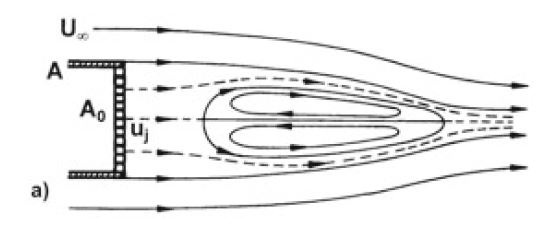
\includegraphics[width=0.5\textwidth]{KorperBearman.jpg}
	\caption{Stumpfk"orper mit Ausblasung von Bearman \cite{Hucho.2011}}
	\label{fig:Bearman}
\end{figure}\\
Die austretende Luft sorgte daf"ur, dass die Str"omungsabl"osung vom K"orperende weggeschoben wurde. Durch die erst sp"ater stattfindende Verwirbelung, f"allt der Widerstand des K"orpers ab.

%-------------------------------------------------------------------------------------
Geropp \cite{Geropp.2000} hat Experimente zur Einblasung am Ende eines Kraftfahrzeuges "uber zwei Schlitze mit Nutzung des Coand\^{a}-Effekts gemacht (\abb{fig:Geropp}).
\begin{figure}[h]
	\centering
	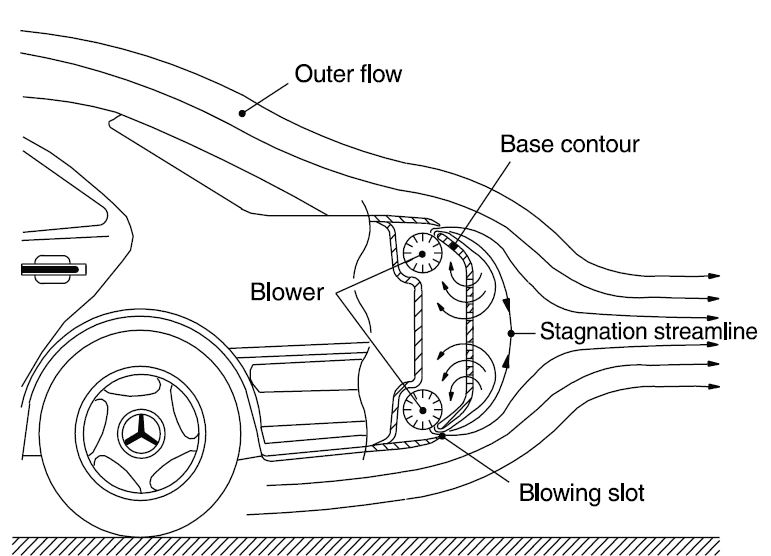
\includegraphics[width=0.5\textwidth]{KorperGeropp.jpg}
	\caption{Stumpfk"orper mit Ausblasung von Geropp \cite{Geropp.2000}}
	\label{fig:Geropp}
\end{figure}\\
Ergebis ist, dass die Ausblasung bei hohen Geschwindigkeiten erfolgen muss, um die Genzschicht zu beeinflussen. Durch den Coand\^{a}-Effekt wird die eingeblasene Luft in das Todwasser umgelenkt, wo sie wieder abgesagt wird. Dadurch wird der Druck hinter dem Fahrzeug erh"oht und der Gesamtwiderstand verrringert. Die Experimente haben gezeigt, dass eine Druckerh"ohung von 50\% und eine Widerstandsverringerung um 10\% m"oglich ist. Au\ss{}erdem wurde ein Energievorteil f"ur moderate Ausblasgeschwindigkeiten mathematisch bestimmt.\\

%--------------------------------------------------------------------------------------
In \cite{Barros.2016} wurde zus"atzlich zu den vorherig beschriebenen Verfahren die Ausblassung gepulst durchgef"uhrt. Dabei soll der Einfluss von Frequenz und Amplitude auf das Widerstandsverhalten untersucht werden.
\begin{figure}[h]
	\centering
	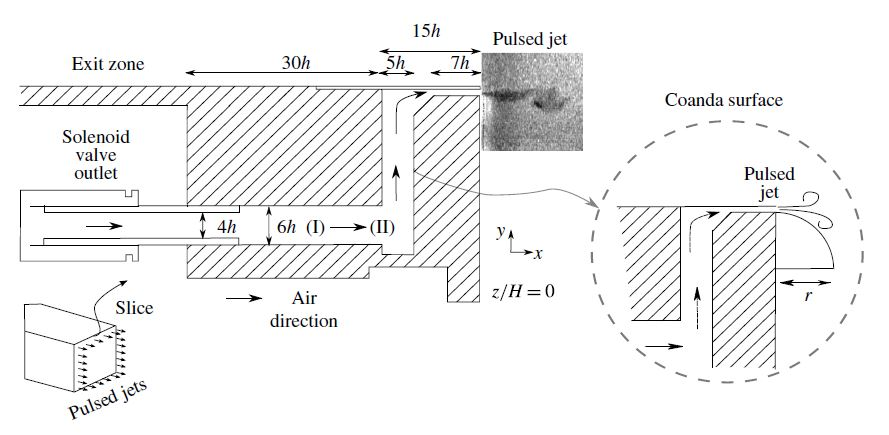
\includegraphics[width=0.8\textwidth]{KorperBarros.jpg}
	\caption{Ausblasung von Barros \cite{Barros.2016}}
	\label{fig:Barros}
\end{figure}\\
In \abb{fig:Barros} ist der schematische Aufbau der gepulsten Ausblasung dargestellt. Diese wird "uber Ventile realisiert, die eine Rechteckkurve mit einem duty cycle (weiter Erl"auterung in \kap{rotierendeWalze}) von 40\% erzeugen. Direkt unter der Ausblasestelle wird zus"atzlich noch eine Coand\^{a}-Fl"ache befestigt.\\
Mit steigenden Frequenzen, aber auch mit einer steigenden Amplitude, wurde eine Umlenkung der Grenzschicht beobachtet. "Uber eine gepulste Einblasung, nahe der nat"urlichen Abl"osefrequenz der Str"omung, konnte der Widerstand am meisten (10\%) gesenkt werden. Bei zus"atzlicher Nutzung der Coand\^{a}-Fl"ache kommt man sogar auf 20\% Widerstandsreduzierung.

%-------------------------------------------------------------------------------------
Modi \cite{MODI.1991} versucht durch drehende Zylinder an einem Truck den Widerstand zu reduzieren.
\begin{figure}[h]
	\centering
	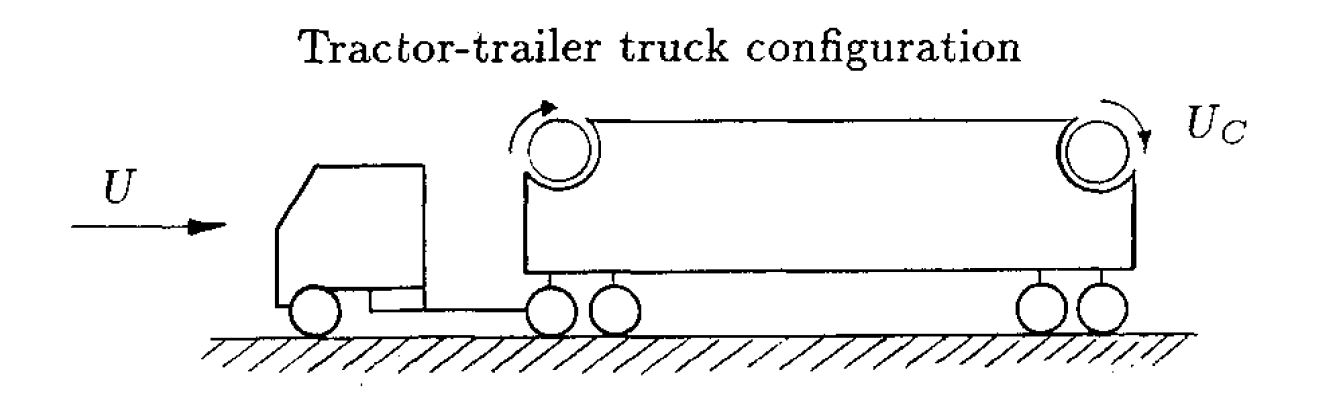
\includegraphics[width=0.6\textwidth]{KorperModi.jpg}
	\caption{Truckmodell von Modi \cite{MODI.1991}}
	\label{fig:Modi}
\end{figure}\\
Dazu sind bei den ersten Windkanalversuchen die Zylinder angeordnet, wie in \abb{fig:Modi} dargestellt. Bei dem ersten Versuch wird die Rauhigkeiten der Zylinder mit durchvariiert. Es gibt einen glatten Zylinder, einen mit einer Rauhigkeit von 40 und einen mit 80. Au\ss{}erdem wird das Verh"altnis der Geschwindigkeiten der Zylinder \(U_c\) bzgl. der Anstr"omgeschwindigkeit \(U\) f"ur alle drei F"alle variiert. Daraus ergeben sich die Widerstandsreduktionen in \tab{tab:Modi}.
\begin{table}[h!]
	\centering
	\begin{tabular}{lrr}
		\toprule
		Zylinder & Widerstandsreduktion [\%] & \(U_c/U\)\\
		\midrule
		glatt & 5 & 2\\
		Rauhigkeit 80 & 10 & 2.1\\
		Rauhigkeit 40 & 13 & 2.1\\
		\bottomrule
	\end{tabular}
	\caption{Widerstandsreduktion bei Modi}
	\label{tab:Modi}
\end{table}\\
Da der hintere Zylinder keinen Impuls in die Grenzschicht einbringen kann und die Versuche das auch best"atigt haben, wurde ein zweites Experiment mit anderer Konfiguration durchgef"uhrt. Dabei wurde ein Zylinder mit spiralf"ormiger Rille in der Oberfl"ache und einer mit einer Vielkeil-Verzahnung, deren Rillen parallel zur Drehachse verlaufen, verwendet. Der erste Zylinder sitzt wie in \abb{fig:Modi} dargestellt, der zweite wurde ans Ende des ersten Drittels der Truckoberseite positioniert.\\
Der spiralf"ormige Zylinder erzielte das gleiche Ergebnis, wie der Zylinder mit einer Rauhigkeit von 40 im ersten Experiment. Der Vielkeil-Verzahnungs Zylinder hat allerdings einen gro\ss{}en Einfluss auf den Widerstand. Wenn man nur den vorderen Zylinder betrachtet k"onnen 29\% Reduktion erreicht werden, beide erreichen bis zu 41\%.

%------------------------------------------------------------------------------------
Alle bisher vorgestellten Verfahren haben nur eine Steuerung des Vorgangs betrachtet. In \cite{Henning.2008} wird jetzt zus"atzlich eine Regelung des Mechanismuses der Str"omungsbeeinflussung beachtet. Dabei m"ochte man "au\ss{}ere St"orungen mit ber"ucksichtigen, die zum Beispiel sich gegenseitig beeinflussende Kraftfahrzeuge aufeinander haben.\\
Im Rahmen der Arbeit wurden unterschiedliche K"orper (\abb{fig:Henning}) analysiert.
\begin{figure}[h]
	\centering
	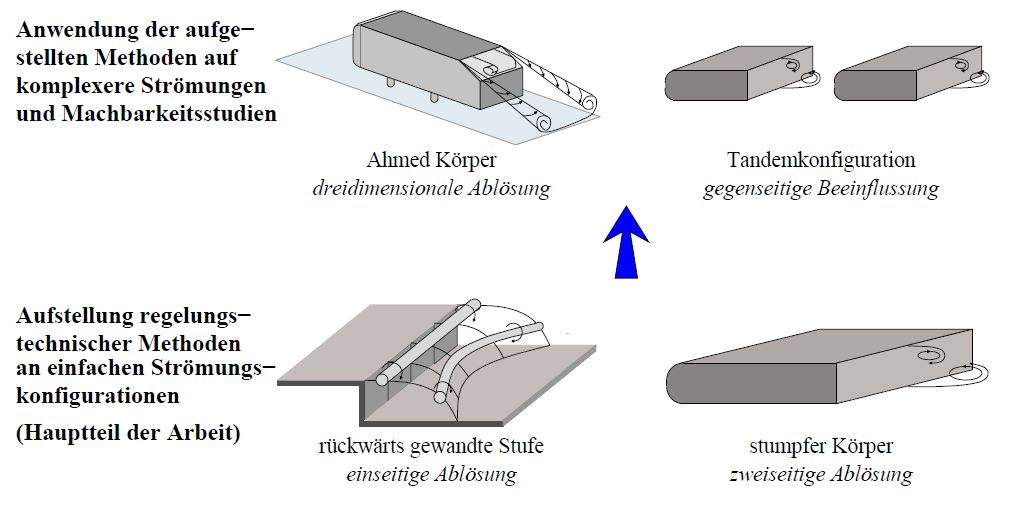
\includegraphics[width=0.8\textwidth]{KorperHenning.jpg}
	\caption{betrachtete Modelle f"ur Auslegung der Regelung \cite{Henning.2008}}
	\label{fig:Henning}
\end{figure}\\
An der r"uck"arts gewandten Stufe wurde erfolgreich die Wideranlegel"ange "uber einen segmentierten Schlitz an der Stufenkante geregelt. Au\ss{}erdem konnte eine Unterdr"uckung von St"orungen erreicht werden. Das Ganze wurde "uber eine Robuste Regelung realisiert.\\
Am stumpfen K"orper wurde mit Hilfe einer Phasenregelung an Ober- und Unterseite eine Widerstandsreduzierung von bis zu 15\% erreicht.\\
Die Tandemkonfiguration wurde im Rahmen einer Machbarkeitsstudie untersucht und f"ur zuk"unftige Arbeiten als sinnvoll betrachtet. Dabei geht es um die St"oreinfl"usse, die der erste K"orper auf den zweiten hat und wie dieser die St"orung "uber eine Regelung beseitigen kann, sodass auch beim zweiten K"orper eine Widerstandsreduzierung m"oglich ist.
